Neste teste foi medido o tempo m�dio gasto com a gera��o de terrenos tanto na \emph{GPU} quanto na \emph{CPU}. Os seguintes par�metros foram utilizados:

\begin{itemize}
\item \emph{Octaves}: Vari�vel (4, 8, 12, 16)
\item \emph{Lacunarity}: 2.5
\item Ganho: 0.5
\item \emph{Offset}: 1.0
\item Tamanho da textura: 512
\item N�mero de divis�es dos quadrados: 150
\item Tamanho dos quadrados: 5.0
\item Fator \emph{LOD}: 2
\end{itemize}



\begin{table}[H]
	\begin{center}
		\begin{tabular}{|c|c|c|}
			\hline
			\emph{Octaves} & GPU & CPU \\
			\hline
			4 & 28,7236 & 46,2948\\
			\hline
			8 & 28,7432 & 92,4299\\
			\hline
			16 & 28,7887 & 187,103\\
			\hline
			32 & 30,1095 & 370,841\\
			\hline
		\end{tabular}
		\caption{Tempo m�dio (em ms) de gera��o dos terrenos, com n�mero vari�vel de \emph{octaves}}
		\label{tabela:geracao}
	\end{center}
\end{table}


A Figura \ref{fig:geracao} apresenta os tempos anteriores.
\begin{figure}[H]
	\center{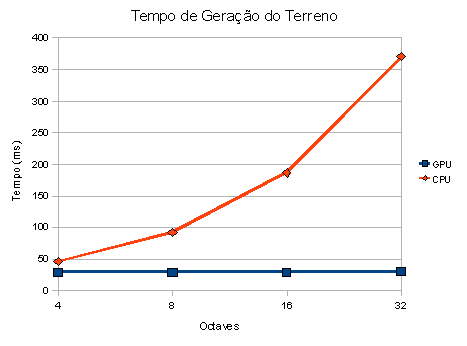
\includegraphics[width=0.4\linewidth]{img/tempoGeracao.png}}
	\caption{\label{fig:geracao} Gr�fico do tempo m�dio (em ms) de gera��o dos terrenos, com n�mero vari�vel de \emph{octaves}.}
\end{figure}


Como pode ser visto, o tempo de gera��o do terreno na \emph{GPU} permanece quase constante, enquanto a gera��o na \emph{CPU} tem um comportamento praticamente linear.
